\documentclass[tikz,border=4pt]{standalone}

\usepackage{amsmath}
\usetikzlibrary{arrows.meta,matrix}

\begin{document}

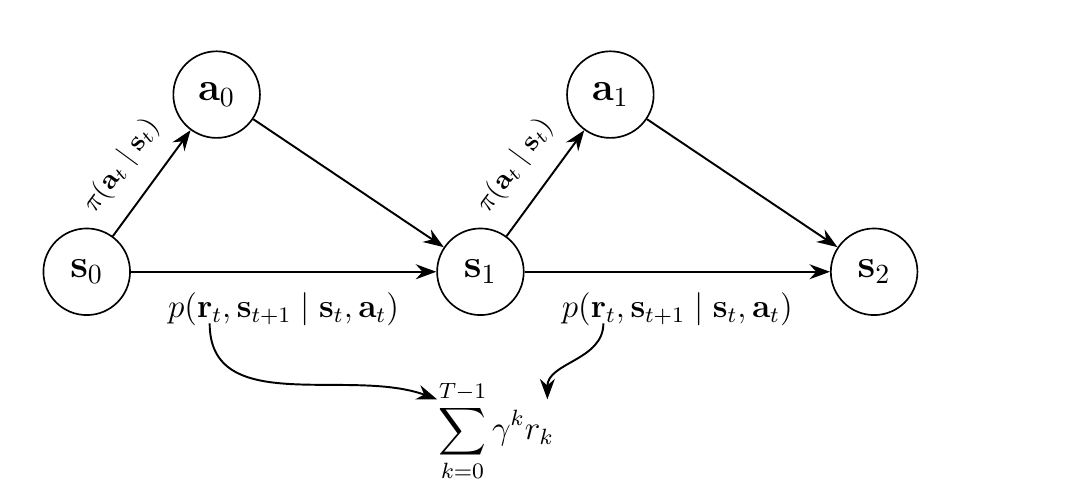
\begin{tikzpicture}[
  node/.style={
    circle,
    draw,
    line width=0.6pt,
    minimum size=11mm,
    inner sep=0pt,
    font=\Large
  },
  edge/.style={
    -{Stealth[length=2.6mm,width=1.9mm]},
    line width=0.7pt
  },
  label/.style={
    inner sep=1.3pt
  },
  objective/.style={
    inner sep=2pt,
    font=\large
  }
]

\path[use as bounding box] (-0.75,-2.55) rectangle (12.30,3.10);
\node[node] (s0) at (0,0) {$\mathbf{s}_0$};
\node[node] (s1) at (5.0,0) {$\mathbf{s}_1$};
\node[node] (s2) at (10.0,0) {$\mathbf{s}_2$};
\node[node] (a0) at (1.65,2.25) {$\mathbf{a}_0$};
\node[node] (a1) at (6.65,2.25) {$\mathbf{a}_1$};
\node[objective] (obj) at (5.20,-2.02)
  {$\displaystyle \sum_{k=0}^{T-1} \gamma^k r_k$};
\coordinate (objleft) at (4.45,-1.62);
\coordinate (objright) at (5.85,-1.62);

\draw[edge] (s0) -- (s1);
\draw[edge] (s1) -- (s2);
\draw[edge] (s0) --
  node[label, pos=0.47, sloped, above=6pt, font=\normalsize]
    {$\pi(\mathbf{a}_t\mid\mathbf{s}_t)$}
  (a0);
\draw[edge] (a0) -- (s1);
\draw[edge] (s1) --
  node[label, pos=0.47, sloped, above=6pt, font=\normalsize]
    {$\pi(\mathbf{a}_t\mid\mathbf{s}_t)$}
  (a1);
\draw[edge] (a1) -- (s2);

\matrix (dyn0) [
  matrix of math nodes,
  nodes={inner sep=0pt, font=\large},
  column sep=0pt,
  row sep=0pt,
  inner sep=1.3pt
] at (2.50,-0.48) {
  p( & |[name=r0term]| \mathbf{r}_t & ,\mathbf{s}_{t+1}\mid\mathbf{s}_t,\mathbf{a}_t & ) \\
};

\matrix (dyn1) [
  matrix of math nodes,
  nodes={inner sep=0pt, font=\large},
  column sep=0pt,
  row sep=0pt,
  inner sep=1.3pt
] at (7.50,-0.48) {
  p( & |[name=r1term]| \mathbf{r}_t & ,\mathbf{s}_{t+1}\mid\mathbf{s}_t,\mathbf{a}_t & ) \\
};

\draw[edge] (r0term.south) to[out=-90,in=160] (objleft);
\draw[edge] (r1term.south) to[out=-90,in=90] (objright);

\end{tikzpicture}

\end{document}
